\documentclass[12 pt]{article}
\usepackage{fancyhdr}
\usepackage[margin = 1 in]{geometry}
\usepackage{amsmath}
\usepackage{enumerate}
% \usepackage{indentfirst}
\pagestyle{fancy}
\usepackage{graphicx}
\usepackage[version=3]{mhchem}
\fancyhf{}
\usepackage{sectsty}	
\lhead{Andrew Wang}
\chead{CS/CNS/EE 155 Machine Learning \& Data Mining}
\rhead{Yue}
\sectionfont{\fontsize{15}{18}\selectfont}
\usepackage{graphicx}
\usepackage{array}
\newcolumntype{P}[1]{>{\centering\arraybackslash}p{#1}}
\newcolumntype{M}[1]{>{\centering\arraybackslash}m{#1}}
\usepackage[font=small,labelfont=bf]{caption}
\usepackage{float}
\usepackage{float}
\usepackage{subfig}
\usepackage{microtype}
\usepackage{ amssymb }
\usepackage{amsmath}
\usepackage{commath}
\begin{document}
	\begin{center}
		\section*{Homework 4}
	\end{center}
	
	
	\subsection*{1 Deep Learning Principles}	
	\noindent\textbf{Question A:}  \\ 
	i. We know that for the second neural network where the weights are initialized to 0, there will be no "learning" because for the back propagation algorithm, we have:
	\begin{equation}
	\frac{\partial S^l}{\partial X^{l-1}} = W^l
	\end{equation}
	
	\noindent In addition, because $ReLU(S) = max(0,S)$, the inputs for any layer after the first will be 0, and the gradient will thus be 0 and so the weights will never be updated. For the first neural network, we have initial non-zero weights, so no issue like this occurs and we see the test error and training error decrease with more iterations.\\
	
	\noindent ii. We first note that with the sigmoid function, we get a non-zero value even when its input is zero (so the problem with all zero initial weights from the previous problem is not relevant). This gives rise to the vanishing gradient problem. The first model takes about 500 iterations before the weights get significantly updated and the second model (with initial weights of zero) has a stagnant error for about 3200 iterations and then starts decreasing after 3200 iterations and the weights get updated correspondingly (in a linear fashion where all weights going from a particular layer are the same). For the first model, it takes ~500 iterations to really start decreasing the error because initially, the weights are very non-significant and with the vanishing gradient problem, the updating of weights is very small with backpropagation. However, after this number of iterations, the initial weights have been updated enough where the gradients become significantly large for backpropagation and error loss. The second model takes much longer because the weights are initially zero so backpropagation takes much longer for these initial weights to become significant, and once the error does start decreasing, it decreases slowly. Also notice that weights from an input all become the same for the second model because they are all set to the same value initially and thus get updated in the same way as we iterate.  \\

	\noindent\textbf{Question B:}  
	
	\noindent As suggested in the hint for this problem, we have the "dying ReLU" problem in the case that we go through all the negative examples first. Due to the ReLU function, when all negative examples are first being fed through, the model get adjusted so much (we develop a heavy negative bias) so that we get correct classification for all these negative points. After this, we get inputs to the ReLU to be negative and due to ReLu's function, future nodes will become zero and "die." Thus, even with the positive examples coming after, learning will fail to occur.   \\
	
	
	\noindent\textbf{Question C:}  \\
	i. 
	\begin{figure}[H]
	\centering
	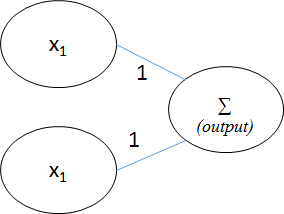
\includegraphics[width=8cm]{OR}
	\end{figure}
	\noindent ii. At the minimum, we need one hidden layer to have one input layer, one hidden layer, and one output layer for three total layers. If we only had one input layer and one output layer, we would simply have a perceptron and we know XOR is not linearly separable (see diagram in lecture slides) and thus unable to be implemented using a perceptron/ neural network with just an input layer and output layer.
	
	\subsection*{2 Depth vs. Width on the MNIST Dataset}
	\noindent\textbf{Question A:} \\ Keras - 1.2.1, Tensorflow - 0.12.1. \\
	
	\noindent\textbf{Question B:} \\ The images are 28 x 28. Each individual value in the array ranges from 0 to 255 and stands for the pixel value (RGB). The new training input size (X$\_$train) is (60000, 784) because there are 60000 images and each image is represented by a list of size 28 x 28 = 784 . The new training output size(y$\_$train) is (60000, 10).\\

	%\begin{figure}[h]
	%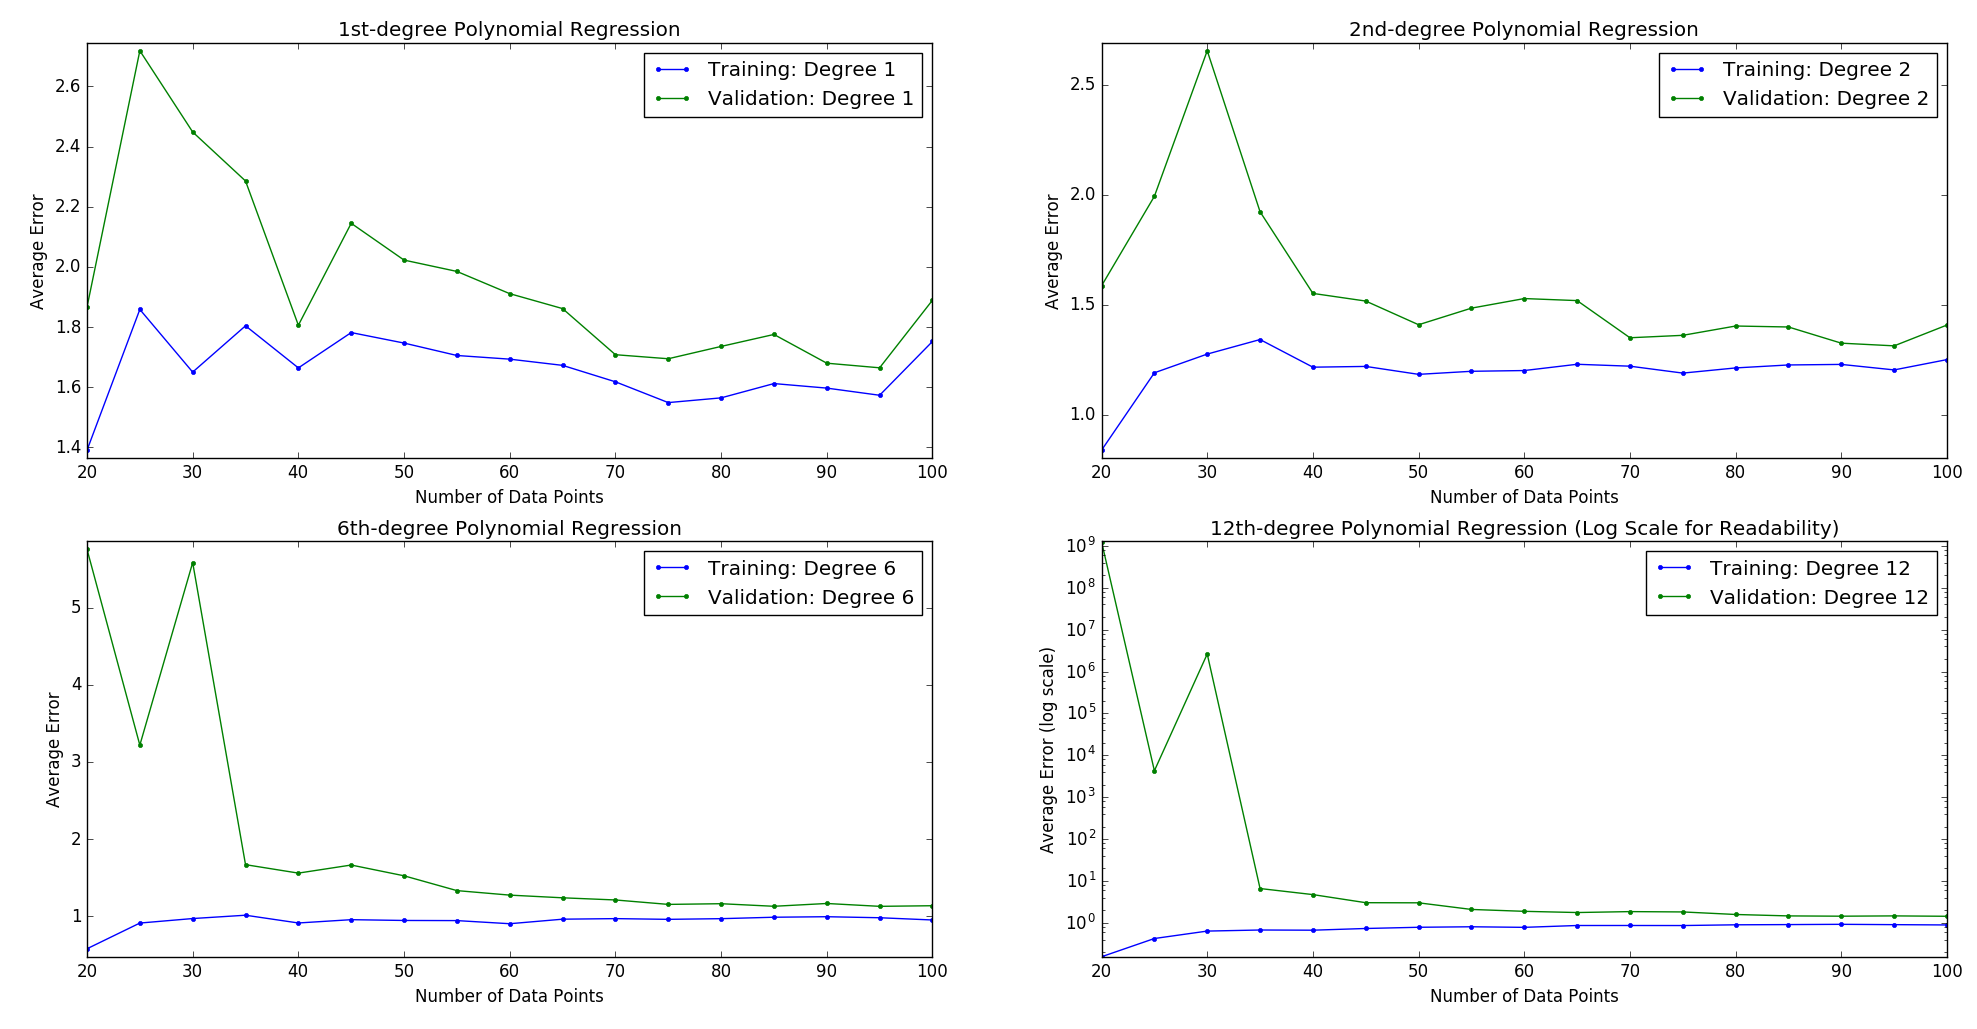
\includegraphics[width=17cm]{LearningCurves}
	%\end{figure}	
	
	\noindent\textbf{Question C:}  \\ See attached code ("MNIST$\_$100.py"). It gave an accuracy of 0.9763. \\
	
	\noindent\textbf{Question D:} \\ See attached code ("MNIST$\_$200.py"). It gave an accuracy of 0.98.\\
	
	\noindent\textbf{Question E:} \\ See attached code ("MNIST$\_$1000.py"). It gave an accuracy of 0.9833.\\

	\subsection*{3 Convolutional Neural Networks}
	\noindent\textbf{Question A:} \\
	Zero-padding allows us to preserve the original size of the image. Ideally, we want to preserve as much information about the original input volume so that we can extract those low level features. The downside of zero-padding is that we could possibly lose important parts of the filter at zero-padded locations. For example, if there are important parts of a feature that are contained on the filter in parts that map to zero-padded positions, then these parts make no contribution. In addition, with zero-padding, the edges of the input image may be weighted differently than the rest of the image such as the center, which may not be desirable. \\

	
	\noindent\textbf{Question B:} \\
	i. 8 filters x 5 x 5 x 3 + 8 biases = 608 parameters. \\
	ii. 8 filters x 28 x 28 x 3 is the shape of the output tensor.\\
	
	\noindent\textbf{Question C:} \\
	i. 
	\[
	\begin{bmatrix}
	1 & 0.5 \\
	0.5 & 0.25
	\end{bmatrix}
	,
	\begin{bmatrix}
	0.5 & 1 \\
	0.25 & 0.5
	\end{bmatrix}
	,
	\begin{bmatrix}
	0.25 & 0.5 \\
	0.5 & 1
	\end{bmatrix},
	\begin{bmatrix}
	0.5 & 0.25 \\
	1 & 0.5
	\end{bmatrix}
	\] \\
	\noindent ii. 
	\[
	\begin{bmatrix}
	1 & 1 \\
	1 & 1
	\end{bmatrix}
	,
	\begin{bmatrix}
	1 & 1 \\
	1 & 1
	\end{bmatrix}
	,
	\begin{bmatrix}
	1 & 1 \\
	1 & 1
	\end{bmatrix},
	\begin{bmatrix}
	1 & 1 \\
	1 & 1
	\end{bmatrix}
	\] \\
	
	\noindent iii. Pooling would be advantageous because pooling allows us to group pixels into regions and then conduct calculations based on these regions. Due to grouping, a missing pixel here and there can be accounted for by its surrounding pixels in the same region as it, and thus the negative effects of such noise can be accounted for. For the case of different angles/location, the noise can similarly be absorbed by surrounding regions of pixels. By pooling, such noise becomes less prominent.\\
	
	
	\noindent\textbf{Question D:} \\
	\noindent i. Without modification, classification loss: 0.16395. For parameters, we have 208 for conv(24x24x8), 3216 for conv(12x12x16), and 2570 for fc(1x1x10). Total is 208 + 3216 + 2570 = 5994 parameters. \\ 
	
	\noindent After modifying the network, and setting num$\_$neurons to 500, I got a classification loss: 0.22775. For fc(1x1x500), we have 288500 parameters, and for fc(1x1x10), we have 5010 parameters, so in total we have 288500 + 5010 =293510 parameters. \\
	
	\noindent ii. We see that each activation highlights a particular outline of the specific input (number) and together, essentially make a "bubble letter" outline of the number. The first activation seems to highlight the right edge between the black number and grey background, the second activation seems to highlight the right edge between the black number and grey background, the third activation seems to highlight the bottom-most edges between the dark letter and grey background, the fourth activation seems to highlight over the main outline of the number, the fifth activation seems to do similar to the second activation but to a greater extent, the sixth activation is very similar to that of the fourth, the seventh activation is highlighting the top edge between number and background, and the eighth activation is highlighting the left edge between number and background. \\ \\
	\noindent Taking all these activations into account, the convolutional layer seems to be trying to learn the general shape of the input/number by detecting the number's edges. \\
	
	\noindent iii. Original validation accuracy: 0.89. \\
	
	 \noindent Modification 1: Changing the stride of one of the pooling layers from 3 to 2 led to an improved validation accuracy of 0.91, (after 10000 training examples). This may be attributed to the fact that before, when the stride was greater, the pooling layer performed excessive down-sampling by reducing the spatial dimensions of the input by too much. The decrease in stride from 3 to 2 may have prevented some of this information loss. \\
	 
	 \noindent Modification 2: Adding a fully connected layer with 20 neurons right before our softmax layer improved the validation accuracy to 0.94 (after 10000 training examples). The fully connected layer is fully connected with the output of the previous layer. At this point, the features have become distinct and learned by all the previous layers. Thus, by feeding the output of these previous layers into a fully connected layer at the end before the final results are outputted, learning is improved. 
\end{document}